\documentclass{math-mech-sci}
\newcommand{\bea}{\begin{eqnarray*}}
\newcommand{\eea}{\end{eqnarray*}}
\newcommand{\be}{\begin{eqnarray}}
\newcommand{\ee}{\end{eqnarray}}


\deftitle%
  {Бустинговый алгоритм дисперсионного анализа на блок-схемах  с медико-биологическими приложениями}

\defauthor%
	{Алексеева Н.П.}%
  {доцент кафедры статистического моделирования СПбГУ, Санкт-Петербург}%
  {nina.alekseeva@spbu.ru}
\defauthor%
  {Подлеснов Я.С.}%
  {студент 4 курса мат-мех факультета, Санкт-Петербург}%
  {st087301@student.spbu.ru}

\begin{document}

\maketitle

\begin{abstract}
В статье изучается проверка значимости факторов линейной модели через бустинговыйй алгоритм, то есть путем многократного применения 
модели дисперсионного анализа на блок-схемах для  несбалансированных ретроспективных данных с последующим изучением распределения полученных статистик.  Определена вариантность  блок-схемы для заданной таблицы сопряженности факторов с учетом  возможной неполноты последней.  Комбинаторным образом получено число  возможных вариантов для полных блок-схем и для типа Q.    Построено два алгоритма  перечисления вариантов, по которым  строятся   статистик проверки значимости влияния сбалансированных факторов.    

\end{abstract}

\section{Введение}

Блок-схема или дизайн $D(v,b,r,k,\lambda)$  определяется как таблица, состоящая из $v$ элементов, сгруппированных по $b$ блокам размера  $k$ так, что каждый элемент встречается  $r$ раз, а каждая пара встречается  $\lambda$ раз. %Если рассматривать число сочетаний из $v$ элементов по  $k$, то получим так называемую полную блок-схему с параметрами $b=C_v^k$.  
Если число блоков меньше $C_v^k$, то такая схема называется неполной сбалансированной. Известны два необходимых соотношения баланса $vr=bk, \lambda(v-1)=r(k-1)$, актуальные для идентификации блок-схем.  В  комбинаторике \cite{bib:holl1970}  большое внимание уделено теоремам существования отдельных блок-схем и методам их построения. В планировании эксперимента с  помощью блок-схем удается существенно снизить число наблюдений при изучении  влияния нескольких факторов типа методов обработки на некоторую  зависимую переменную.  Для того чтобы уменьшить число наблюдений,  разные методы обработки при различных  условиях применяются по специальной схеме.  Дисперсионному анализу на  блок-схемах  посвящена классическая  монография \cite{bib:duge1972}. 

Идея данной работы состоит в том, чтобы применить этот метод на ретроспективных данных с большим числом градаций. Для этого предполагается проводить дисперсионный анализ на частичных подвыборках, градации факторов которых образуют блок-схему,  а вывод о значимости факторов осуществлять  по  ансамблю полученных статистик.   
Этим  объясняется термин бустинговость, поскольку общий вывод осуществляется на основе анализа повторяемости заведомо более слабых выводов по фрагментам выборки. 
Задача заключается, с одной стороны, выборе подходящей блок-схемы, с другой стороны, в оценке числа вариантов ее применения. Ответы на эти вопросы в большей степени определяются типом выбранной блок-схемы  и ее комбинаторными свойствами. 

	\section{Об отборе сбалансированных данных }


В табл.	\ref{tab1} представлены данные о среднем проценте пораженных легких у больных ковидом в зависимости от возрастной группы и порогового уровня белка острой фазы \footnote{Белок острой фазы или СРБ возрастает в организме при наличии воспалительного процесса}. Для краткости столбцы, которые отражают возрастную группу, пронумерованы от 0 до 5. Строки таблицы также  перенумерованы от нуля до девяти, а в последней строке указаны номера подчеркнутых строк. В каждой строке, отвечающей некоторому уровню белка СРБ, подчеркнуты какие-то три значения. Если рассмотреть  номера столбцов с подчеркнутыми значениями (столбец  $b_j$), то можно непосредственно убедиться в том, что номера шести столбцов, сгруппированные по три в 10 блоков, образуют блок-схему $D(6,10,5,3,2)$.  
%
В качестве геометрической иллюстрации   дизайна  $D(6,10,5,3,2)$ можно рассматривать пятиугольник, вершины которого соединены с центром. Пять внутренних треугольников образуют пять блоков. Остальные пять блоков представляют собой треугольники со стороной в виде ребра пятиугольника, соединенного с противоположной вершиной (рис. \ref{fig:penta}).  
%


Наблюдения с выделенными  сочетаниями факторов образуют сбалансированную частичную подвыборку,  для которой может  быть применен   дисперсионный анализ на блок-схемах. 

\begin{table}[ht]\centering\begin{tabular}{rrrrrrr|r}  
		
		\hline 
		возраст
		& [22,44]~0 & (44,55] & (55,65] & (65,76] & (76,87] & (87,98] &  $b_j$\\  \hline
		CRB  & 0 & 1& 2& 3 & 4 & 5 & \\   \hline
		
		(0,2.5]~0 & \underline{19} & \underline{21} & 25 & 36 & 47 &  \underline{10} &	015\\  
		(2.5,2.85]~1& 16 &  \underline{10}& \underline{28} &  &  &  \underline{10} & 125 \\  
		(2.85,3.2]~2 &  \underline{20}&  & \underline{30} & 38 &  \underline{60} &  & 024 \\  
		(3.2,3.55]~3 & 45 & 28 & \underline{40} & \underline{31}& 29 & \underline{28}  & 235 \\ 
		(3.55,3.9]~4& 58 & 88 & 60 &\underline{53} & \underline{36} & \underline{16}  & 345\\  
		
		(3.9,4.25]~5 & {50} & \underline{48} & {61} & \underline{68}& \underline{36} & & 134 \\  
		(4.25,4.6]~6 & \underline{43} & 43 & 60 & 71 & \underline{59} & \underline{65}   &045\\  
		(4.6,4.95]~7 & \underline{85} & 64 & \underline{77} & \underline{72}& 56 & 55 & 023\\   
		(4.95,5.3]~8 & \underline{15} & \underline{69} & 68 & \underline{70} & 76 & 39 & 013\\   
		(5.3,5.65]~9 &  & \underline{66} & \underline{76} & 35 & \underline{25} &  &124\\   \hline
		$\gamma_i$  &  02678& 01589 & 12379&  34578& 24569& 01346 &\\   
		\hline\end{tabular}
	\caption{Средний объем поражения легких  в зависимости от уровня белка CRB и от возраста больных ковидом.}\label{tab1}\end{table}

\section{Дисперсионный анализ на блок-схемах }

Модель дисперсионного анализа на блок-схемах применяется для сбалансированной выборки и имеет вид 
\bea
x_{ij}=\mu+v_i+b_j+\varepsilon_{ij},~~\varepsilon_{ij}\sim {\cal N}(0,\sigma)\,,
\eea
где через $v_i$ и $ b_j$ обозначены дифференциальные эффекты факторов, указанных соответственно в строках и столбцах таблицы  \ref{tab1}. 
Основные статистики -- это суммы по строкам 
$
V_i=\sum\limits_{j}x_{ij}
$
и по столбцам
$
B_j=\sum\limits_{i}x_{ij},
$ а также сумма $T_i=\sum\limits_{j\in \gamma_i }B_j$.  
Оценки параметров по методу наименьших квадратов  \cite{bib:duge1972} имеют вид
\bea 
\hat{\mu}=\frac{1}{bk}\sum\limits_{i,j} x_{ij},~~
%
\hat  v_i=\frac{kV_i-T_i}{\lambda v},~~
%
\hat {b}_j=\frac 1 k (B_j-\sum\limits_{i\in b_j} \hat v_i )-k\hat \mu\,,
\eea
где суммирование $(i,j)$  означает или $\sum\limits_{i=1}^v\sum\limits_{j\in \gamma_i}$, или 
$\sum\limits_{j=1}^b\sum\limits_{i\in \beta_j}$, а $b_j$ и  $\gamma_i$ соответственно блоки прямого $(b_j)$и двойственного $(\gamma_i)$  дизайна\footnote{Двойственный дизайн образуют блоки прямого дизайна, взятые в качестве элементов, агрегированные по инцидентности отдельного элемента прямого дизайна.} (табл.\ref{tab1}).
%
Статистические критерии опираются на разложение суммы квадратов отклонений $ \sum\limits_{i,j}(x_{ij}-\hat{\mu})^2=S^2_e+S^2_v+S^2_b,$ где
\bea
%
S_v^2=\sum\limits_{ij}\left(\hat v_i-\frac{1}{k}\sum\limits_{i\in \beta_j}\hat v_i\right)^2,~
S_b^2=\sum\limits_{j=1}^b k\left( \frac{B_j}{k}-\hat{\mu}^2\right)^2, \\
S_e^2=\sum\limits_{i,j}\left(x_{ij} - \hat v_i +\frac 1 k \sum\limits_{l\in b_j}\hat v_i -\frac{B_j}k\right)^2\,.
\eea
При справедливости  гипотез о незначимости факторов статистики
\bea
F=\frac{S_v^2}{S_e^2}\cdot \frac{bk-v-b+1}{v-1}~~\mbox{и} ~~F=\frac{S_b^2}{S_e^2}\cdot \frac{bk-v-b+1}{b-1}
\eea
имеют распределение Фишера соответственно с $df_v=v-1$, $df_e=bk-v-b+1$ и с $df_b=b-1$, $df_e=bk-v-b+1$ степенями свободы.
\section{Комбинаторный аспект вариантности дизайна}





Очевидно в таблицу с $b$ строками и $v$ столбцами можно вписать очевидно  дизайн с $v$ элементами и $b$ блоками.  
Из  табл. \ref{tab1} имеем $v=6$  на  $b=10$. Известен  дизайн $D(6,10,5,3,2)$ с таким соотношением числа элементов и числа блоков   \cite{bib:holl1970}. Он  является остаточным для блок-схемы $D(11,5,2)$ типа $Q$\footnote{ К типу  Q относятся блок схемы, у которых орбита представляет собой квадратичные вычеты по полю  $F_q$.  Например, для $q=11$ квадратичными вычетами являются числа 1, 3, 4, 5, 9. Если построить одиннадцать блоков вида  $(1+j, 3+j, 4+j, 5+j, 9+j)$, где $j=0,1,\ldots,10$, то получим дизайн $D(11,11,5,5,2)$, остаточным к которому оказывается  $D(6,10,5,3,2)$. }.
%		
%
Группой  автоморфизмов\footnote{Подстановка на элементах блок-схемы $D$, относительно которой инвариантно множество блоков, называется  автоморфизмом дизайна. 

} 
дизайна $D(6,10,5,3,2)$  является группа  $PSL_2^{F_5}$  симметрий додекаэдра.  \footnote{В $PSL_2^{F_5}$ буква   $L$ означает, что это линейная группа матриц, индекс 2 ---  порядка два над полем $F_5$  с единичным определителем ($S$). В проективной  группе  $(P)$    матрицы, отличающиеся сомножителем, задают одно и то же преобразование.}   Элементам этой группы  соответствуют  способы расстановки вершин графа (рис.\ref{fig:penta})  с сохранением  блоков. 
Например, в центр можно поставить любой из шести элементов,  пусть 5, вершину 0 можно обозначить оставшимися пятью способами, а для обозначения вершины 1 остаются только два варианта: либо 1, либо 4, так как пара 05 входит в состав двух блоков 015 и 045. Для оставшихся  вершин все однозначно.  Таким образом получаем $60=6\cdot 5\cdot 2$ автоморфизмов. 

\begin{figure}
	\centering
	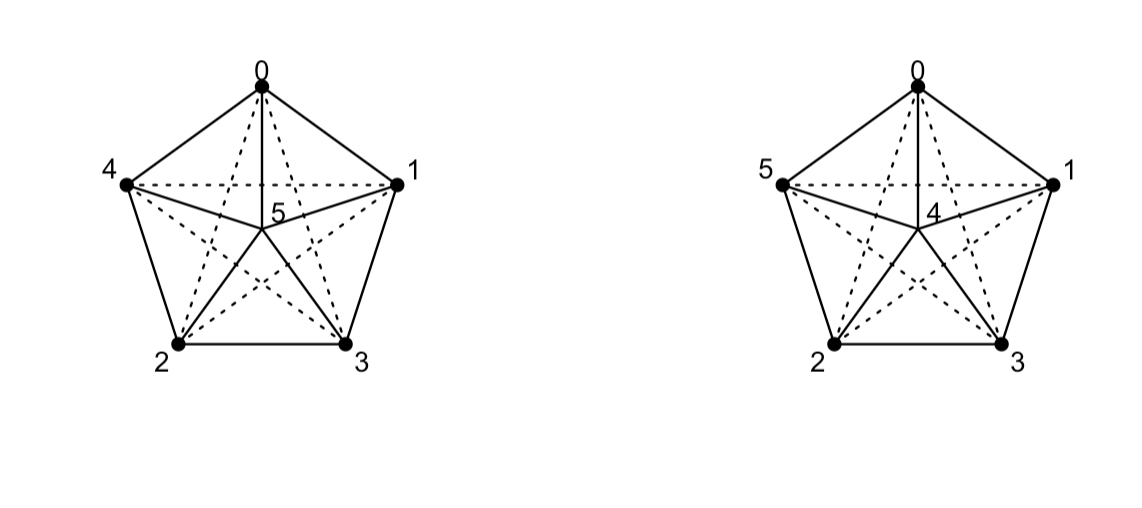
\includegraphics[width=0.7\linewidth]{penta2}
	\caption{ Геометрическая интерпретация неавтоморфных подстановок дизайна $D(6,10,5,3,2)$.}
	\label{fig:penta}
\end{figure}

Неавтоморфными  будем называть  подстановки с неодинаковыми  множествами блоков\cite{bib:alex2012}.  
Для того чтобы вычислить $S_D$ число неавтоморфных подстановок дизайна, нужно  $v!$ подстановок на элементах разделить на число его автоморфизмов. Например, дизайн $D(6,10,5,3,2)$ имеет 
$
S_D=\frac{6!}{60}=12
$
неавтоморфных подстановок. Очевидно половина подстановок являются противоположными, а шесть  неавтоморфных подстановок можно получить, если зафиксировать, к примеру, тройку элементов 0, 1,  5, а на оставшихся трех 2, 3, 4 задать шесть подстановок (рис. \ref{fig:penta}).  




Итак, если в  матрице наблюдений типа табл.\ref{tab1} выбрать   $b$ строк и $v$ столбцов так, что   $r$ элементов встречаются  в каждом столбце и $k$ элементов в каждой строке, а каждая пара встречается $\lambda$  раз, то мы получаем сбалансированную решетку в виде некоторой подстановки дизайна $D(v,b,r,k,\lambda)$ с упорядоченными блоками. Совокупность всех вариантов вложения дизайна в таблицу (учитываются только ненулевые ячейки), будем называть вариантностью. Полный порядок  вариантности  определяется числом неавтоморфных подстановок, умноженных на число перестановок блоков, то есть $b! \cdot S_D$. 


\section{Алгоритмический аспект  вариантности дизайна}

Поскольку в реальности матрица наблюдений редко представлена полным набором всевозможных сочетаний градаций факторов,  число решеток оказывается намного меньше $b!\cdot S_D$.  Например, во второй строке таблицы \ref{tab1}  представлены только элементы $0,1,2,5$. Поэтому  во второй строке могут быть только два блока $B_0=015$  и  $B_1=125$.   Аналогично в третьей строке с элементами $0,2,3,4$ могут располагаться только блоки  $B_2=024$  и  $B_7=023$, а в десятой строке с элементами $1,2,3,4$ могут располагаться только блоки  $B_5=134$  и  $B_9=124$. Еще в шестой  строке отсутствует элемент 5, поэтому там могут располагаться пять  блоков, которые этого числа не содержат, $024, 134, 023, 013$  и $124$. Заметим, что в трех строках с пропущенными двумя элементами  могут располагаться разные блоки, поэтому рассматривая восемь всевозможных их сочетаний, увидим, что обязательно два из них не содержат элемент  $5$, следовательно, получаем число перестановок блоков в этом одном из 12 дизайнов в виде  $2^3\cdot 3\cdot 6!=24\cdot 6!=17280$. 
Аналогично считаются перестановки блоков для остальных одиннадцати подстановок.
Всего для такой структуры распределения по градациям получено  $(4\cdot 24 +2\cdot 20  +4\cdot  15 +2\cdot 18)\cdot 6!=232\cdot 6!=167040$, что более чем в 250 раз меньше полного числа перестановок. В целом, процесс алгоритмизуется, и можно непосредственно убедиться в правильности подсчета числа необходимых решеток. 

Для контроля  был реализован еще один алгоритм, основанный на расстановке всевозможных вариантов блоков. 
На первых двух этапах все просто - выбираем первый  $B_1$ блок $20=C_6^3$ способами, второй  $B_2$ восемнадцатью, поскольку исключаются первый блок и ему противоположный.  Далее сложнее, поскольку из 16-ти   вакантных для $B_3$  блоков, которые определяются парой $B_1,B_2$,   не все тройки блоков  возможны. 
Но  можно построить алгоритм, по которому на  $n$-м  шаге проверяется, в какие подстановки дизайна входят  блоки $B_1,\ldots,B_n$, $0<n\leq {b-1}$. Если такой дизайн один, то процедура заканчивается приведением  всех оставшихся перестановок ${\cal P}(B_{n+1},\ldots,B_b)$. Иначе рассматриваются возможные кандидатуры на $B_{n+1}$. Для этого из множества элементов $\Omega_v$ дизайна исключаются предыдущие блоки  $B_1,\ldots,B_n$ и им противоположные. Если представлены не все ячейки таблицы сопряженности по градациям факторов, то нужно рассматривать пересечение с множеством возможных блоков, вызванном неполнотой данных.  
Реализованный алгоритм в R алгоритм привел все $S_D\cdot b!$ необходимых подстановок, но с большим преимуществом во временных затратах. 





\section{Практические примеры }

Для таблицы сопряженности факторов \ref{tab1}, в которой  $b=10$  строк и $v=6$ столбцов, в случае полного перебора необходимо перебрать 
43545600 решеток  дизайна $D(6,10,5,3,2)$. Если заранее учитывать незаполненность некоторых  ячеек, число вариантов сводится, как было указано ранее,  к 
167040. Для каждого варианта  вычислены статистики Фишера и оценены значимости влияния факторов. Установлена высокая значимость влияние белка СРБ на процент поражения легких,  в $ 93.36\%  $ $p$-значение не превышает уровень значимости $\alpha=0.1$, в $ 80\%  $  уровень значимости $\alpha=0.05$, в то время как фактор возраста в  $95\%$ случаев оказался незначимым.

Второй пример связан с исследованием влияния разных методов лечения ожогов у лабораторных крыс. В качестве зависимой переменной рассматривалась площадь ожога, а  в качестве факторов рассматривались способ лечения с 4-мя градациями и масса тела как показатель состояния всего организма с 6-ю градациями. 
Для отбора частичных выборок использовали  дизайн $D(4,6,3,2,1)$ -- полную блок-схему с единственной подстановкой. Были проанализированы распределения значимостей соответствующих статистик. В результате удалось  выделить два существенных временных момента: 10 и 19 дней. Через 10 дней проявилось наибольшее различие между методами лечения, а через 19 дней проявилась наибольшая дифференциация по массе. 




\section{Заключение}


Таким образом, сопоставляя таблицу сопряженности факторов с  комбинаторными свойствами адекватных блок-схем, можно  заранее оценить число возможных статистических итераций бустингового алгоритма.   
Показана целесообразность изучения комбинаторных свойств дизайнов и двойственный подход в параметризации 
вариантности дизайнов. В дальнейшем предполагается расширить алгоритм на блок-схемы других типов и изучить свойства нового  критерия на модельных данных. 


\bibliographystyle{ugost2008}
\bibliography{Sources}
\addcontentsline{toc}{section}{Список литературы}
\renewcommand\refname{Литература}

\end{document}
